\section{Descrição do Problema}

\subsection{Grafos e Redes Muiltimodais}

\frame
{
\frametitle{Definição de Grafo}
\begin{block}{Definição}
``Um grafo é uma representação abstrata de um conjunto de objetos, onde alguns pares de objetos estão conectados por ligações.
Os objetos representados por abstrações matemáticas chamadas vértices, e as ligações que conectam alguns dos pares de vértices são chamadas de arestas.''
\\ ~ \\
\tiny
Fonte: Wikipedia, Graph (Mathematics). Tradução própria.
\end{block}
}

\frame
{
\frametitle{Exemplo de Grafo}
\begin{columns}[c]
\column{1.5in}
	\begin{exampleblock}{Exemplo}
		$G = (V,E)$ \\
		$ $ \\
		$V = \{1,2,3,4\}$ \\
		$ $ \\
		$E = \{e_1,e_2,e_3,e_4\}$ 
	\end{exampleblock}
\column{1.5in}
	\begin{figure}
		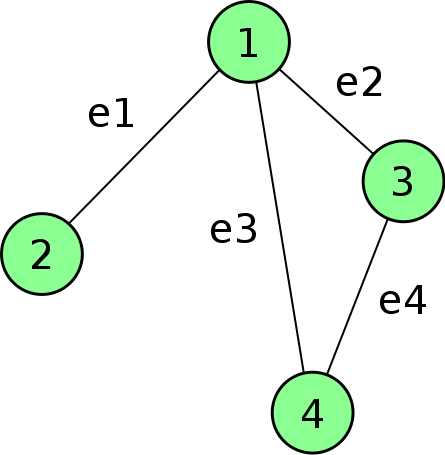
\includegraphics[width=\textwidth]{./imgs/grafo.png}
		\caption{Exemplo de grafo}
		%TODO: ref
		%\fonte{\citeonline{wikigrafo}}
	\end{figure}
\end{columns}
}

\frame
{
\frametitle{Definição de rede Multimodal}
\begin{block}{Definição}
Uma rede multimodal é um grafo cujas arestas tem pesos, direção e modo. A direção determina que cada aresta tem um nó de origem e um nó de destino.
Os pesos são valores positivos associados à cada aresta. Cada aresta tem também um modo associado dentre um conjunto finito de modos. Portanto, os modos particionam o conjunto das arestas.
\end{block}
}

\frame
{
\frametitle{Exemplo de Rede Multimodal}
	\begin{figure}
		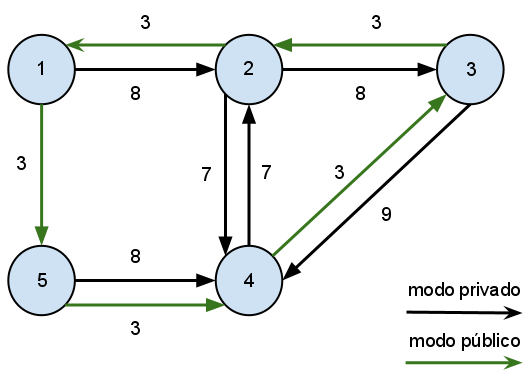
\includegraphics[width=.8\textwidth]{./imgs/multimodal.png}
		\caption{Exemplo de rede multimodal}
	\end{figure}
}

\subsection{Redes de Transporte e o Problema do Caminho mínimo}
\frame
{
\frametitle{Definição de Rede de Transporte}
\begin{block}{Definição}
Uma rede de transporte é uma rede multimodal onde as arestas, ao invés de pesos, tem dois valores, o tempo de partida e o tempo de chegada. Um caminho através de uma rede de transporte tem um horário inicial definido, e as arestas só podem ser atravessadas no tempo de partida, e só terminam de ser atravessadas no tempo de chegada.
\end{block}
}

\frame
{
\frametitle{Exemplo de Rede de Transporte}
	\begin{figure}
		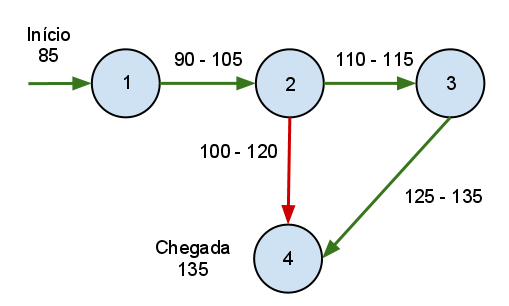
\includegraphics[width=.8\textwidth]{./imgs/redetransporte.png}
		\caption{Exemplo de rede de transporte}
	\end{figure}
}

\frame
{
\frametitle{O Problema do Menor Caminho em uma Rede de Transporte Multimodal}
\begin{exampleblock}{Entradas}
	\begin{itemize}
	\item Nó de origem.
	\item Nó de destino.
	\item Horário de início.
	\end{itemize}
\end{exampleblock}

\begin{alertblock}{Saídas}
	\begin{itemize}
	\item Horário mínimo de chegada.
	\item Caminho que resulta no horário mínimo de chegada.
	\end{itemize}
\end{alertblock}
}

\frame
{
\frametitle{Algoritmo de Caminho Mínimo}
Modificação do algoritmo de Dijkstra para contemplar restrições adicinais:
	\begin{itemize}
	\item Tabela de itinerários.
	\item Tempo de espera.
	\item Tratamento diferente de cada modo.
	\item Tempo de ``folga'' em troca de modo ou serviço.
	\end{itemize}
}
